\documentclass[10pt,a4paper]{article}
\usepackage[utf8]{inputenc}
\usepackage[T1]{fontenc}
\usepackage[spanish]{babel}
\usepackage{amsmath,amssymb}
\usepackage{graphicx}
\usepackage{float}
\usepackage{booktabs}
\usepackage{geometry}
\usepackage{listings}
\usepackage{xcolor}
\usepackage{hyperref}
\usepackage{caption}
\usepackage{setspace}
\usepackage{enumitem}
\usepackage{multirow}
\usepackage[round]{natbib}

\geometry{top=1.5cm, left=1.5cm, right=1.5cm, bottom=2cm}

\singlespacing

\setlength{\parskip}{3pt}
\setlength{\parindent}{0pt}

\lstset{
  language=R,
  basicstyle=\ttfamily\footnotesize,
  backgroundcolor=\color{gray!8},
  frame=single,
  breaklines=true,
  keywordstyle=\color{blue!70!black},
  commentstyle=\color{green!50!black},
  stringstyle=\color{red!70!black},
  numbers=left,
  numberstyle=\tiny\color{gray},
  numbersep=5pt,
  xleftmargin=1.5em,
  framexleftmargin=1em
}

\hypersetup{colorlinks=true, linkcolor=blue!60!black, citecolor=blue!60!black, urlcolor=blue!60!black}
\pagestyle{plain}

\begin{document}

\begin{center}
{\LARGE \textbf{Control 4: Selección de número de agrupamientos con K-Medias}}\\[4pt]
{\normalsize Juan Muñoz, Vicente Rivera, Fernando Valdés}\\[2pt]
{\small juan.munozveloso2023@alu.uct.cl, vrivera2023@alu.uct.cl, fvaldes2023@alu.uct.cl}\\[2pt]
{\small Control 4, INFO1184, Semestre I-2026}
\end{center}

\section*{Resumen}

En este control se analiza el conjunto \texttt{wine.data} mediante k-means para comparar valores de $k$ entre 2 y 15. En la Pregunta 1, la elección del número de grupos se realiza únicamente desde centroides y visualización, usando proyección PCA y evidencia numérica descriptiva de separación y fragmentación, sin aplicar métricas de calidad de clustering. En la Pregunta 2, se utiliza el método del codo con la suma de cuadrados intra-cluster (WSS). Los resultados muestran un quiebre principal al pasar de $k=2$ a $k=3$ y, desde $k=4$, mejoras marginales asociadas a sobre-segmentación. Por ambas vías de análisis, se concluye que el valor más adecuado para este dataset es $k=3$.

\section{Introducción}

El algoritmo k-means es una técnica de aprendizaje no supervisado que particiona un conjunto de observaciones en $k$ grupos buscando alta similitud intra-cluster y separación inter-cluster. Su objetivo puede expresarse mediante la minimización de la suma de cuadrados intra-cluster:
\begin{equation}
\text{WSS}(k) = \sum_{j=1}^{k} \sum_{x \in C_j} \|x - \bar{x}_{C_j}\|^2,
\label{eq:wss}
\end{equation}
donde $\bar{x}_{C_j}$ corresponde al centroide del cluster $C_j$.

En clases de semana 6 se revisó que la selección de $k$ puede sustentarse tanto en criterio visual como en el método del codo \citep{levano2026}. El presente trabajo aplica ambos enfoques al set de vinos de UCI (178 observaciones, 13 variables continuas), estandarizando variables para evitar sesgo por escala \citep{aeberhard1991}.

\section{Desarrollo}

\subsection{Preparación de datos y configuración experimental}

Se cargó \texttt{wine.data}, separando la etiqueta de clase original y usando solo variables numéricas para el agrupamiento. Luego se estandarizaron las 13 variables y se ejecutó k-medias para $k \in \{2,\dots,15\}$ con \texttt{set.seed(101)}, \texttt{nstart=100} e \texttt{iter.max=200}. El script completo se presenta en el \hyperref[anx:script]{Anexo A.2}.

\subsection{Pregunta 1: Comparación por centroides y visualización}

Siguiendo estrictamente el enunciado, esta pregunta se responde sin usar método del codo ni índices clásicos de calidad de clustering. La evaluación se realizó mediante: (i) visualización de grupos y centroides en PCA (\hyperref[fig:pca]{Fig.~\ref*{fig:pca}}), y (ii) análisis descriptivo de distancia mínima entre centroides y tamaño del clúster menor (\hyperref[fig:diagdist]{Fig.~\ref*{fig:diagdist}} y \hyperref[fig:diagsize]{Fig.~\ref*{fig:diagsize}}).

\begin{table}[H]
\centering
\footnotesize
\begin{tabular}{c c c c}
\toprule
$k$ & Dist. mín. entre centroides & Clúster más pequeño & Lectura descriptiva \\
\midrule
2 & 3.827 & 87 & Partición gruesa \\
3 & 3.586 & 51 & Tres grupos bien definidos \\
4 & 2.705 & 28 & Subdivisión adicional \\
6 & 2.535 & 4 & Fragmentación marcada \\
10 & 1.789 & 3 & Sobre-segmentación \\
15 & 1.873 & 2 & Micro-clusters inestables \\
\bottomrule
\end{tabular}
\caption{Indicadores descriptivos basados en centroides para valores representativos de $k$.}
\label{tab:p1centroides}
\end{table}

La Tabla~\ref{tab:p1centroides} y la \hyperref[fig:pca]{Fig.~\ref*{fig:pca}} muestran que con $k=3$ se obtiene una estructura interpretable y estable; para $k \ge 6$ aparecen grupos muy pequeños y cercana superposición de centroides, lo que dificulta la interpretación global.

\textbf{Respuesta Pregunta 1:} basándose solo en centroides y visualización, el número óptimo observado es \textbf{$k=3$}.

\subsection{Pregunta 2: Método del codo}

Para esta pregunta se aplicó el método del codo sobre WSS total (ec.~\ref{eq:wss}) para $k=2..15$.

\begin{table}[H]
\centering
\footnotesize
\begin{tabular}{c c c}
\toprule
$k$ & WSS & Disminución porcentual respecto a $k-1$ \\
\midrule
2 & 1649.44 & --- \\
3 & 1270.75 & 22.96\% \\
4 & 1168.61 & 8.04\% \\
5 & 1095.15 & 6.29\% \\
6 & 1032.80 & 5.69\% \\
7 & 975.92 & 5.51\% \\
\bottomrule
\end{tabular}
\caption{Resumen del método del codo (extracto $k=2$ a $k=7$).}
\label{tab:elbow}
\end{table}

El mayor quiebre ocurre de $k=2$ a $k=3$ (22.96\% de reducción), y desde $k=4$ las mejoras pasan a ser menores y decrecientes. La curva completa se observa en la \hyperref[fig:elbow]{Fig.~\ref*{fig:elbow}}.

\textbf{Respuesta Pregunta 2:} por método del codo, el número óptimo de agrupamientos es \textbf{$k=3$}.

\section{Reflexión}

Este control permitió justificar la selección de $k$ desde dos perspectivas complementarias: criterio geométrico (centroides y visualización) y criterio de compactación (WSS-codo). En este caso, ambos enfoques convergen en $k=3$, reforzando la validez de la decisión.

De forma general, el trabajo también permite observar que la decisión sobre el número de clusters no debe basarse solo en reducir error interno, sino en conservar interpretabilidad de los grupos. Cuando $k$ aumenta demasiado, aparecen micro-clusters que disminuyen la utilidad analítica del resultado y dificultan su traducción a decisiones de negocio.

Finalmente, la experiencia práctica en R consolida lo visto en clases: estandarizar variables, fijar semilla, comparar escenarios de $k$ y respaldar conclusiones con evidencia numérica y visual son pasos necesarios para un análisis de conglomerados técnicamente sólido y comunicable en un informe técnico.

\bibliographystyle{apalike}
\bibliography{referencias}

\newpage
\section*{Anexo}

\subsection*{A.1 Figuras generadas}
\phantomsection\label{anx:figuras}

\begin{figure}[H]
  \centering
  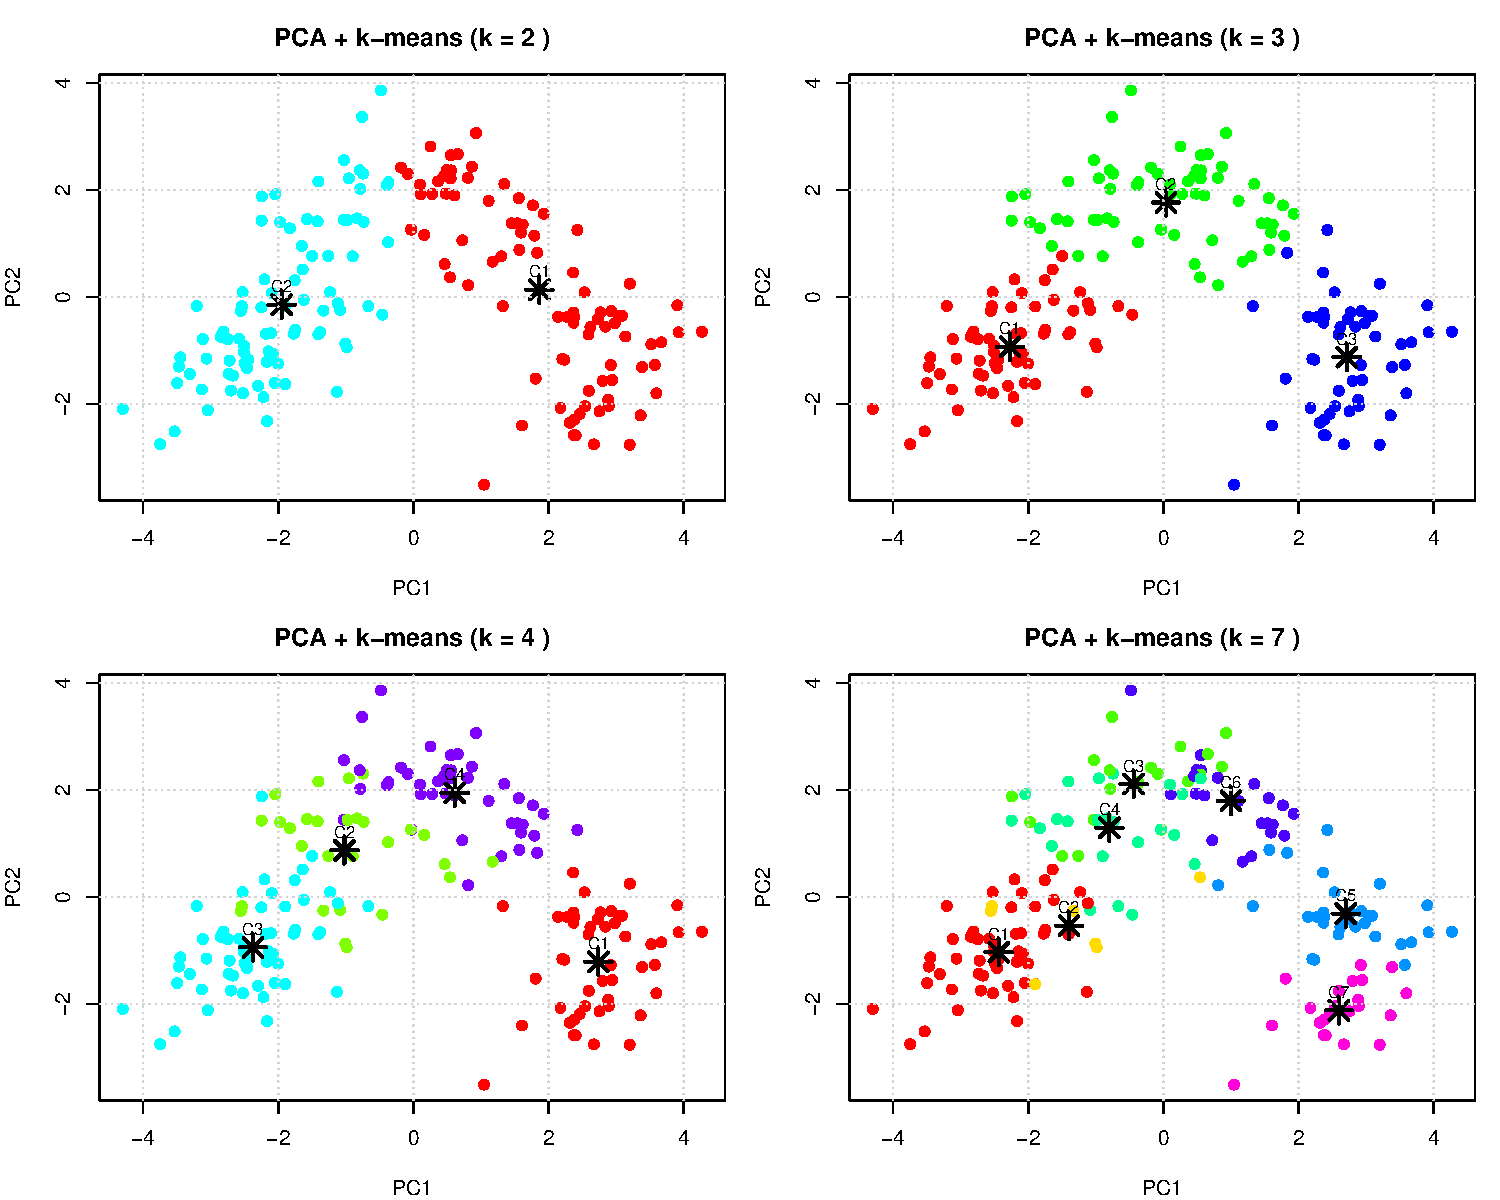
\includegraphics[width=0.78\textwidth]{cc4_pca_k2_k3_k4_k7.pdf}
  \caption{Visualización PCA con centroides para $k=2,3,4,7$.}
  \label{fig:pca}
\end{figure}

\begin{figure}[H]
  \centering
  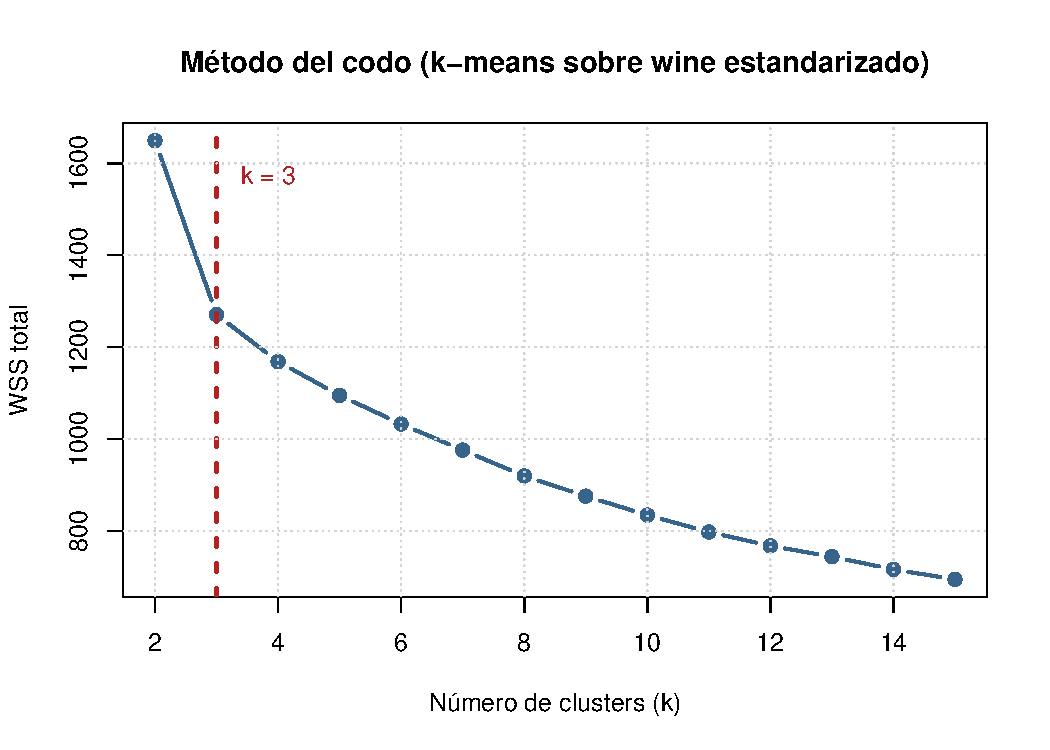
\includegraphics[width=0.75\textwidth]{cc4_elbow_wss.pdf}
  \caption{Método del codo para $k=2,\dots,15$.}
  \label{fig:elbow}
\end{figure}

\begin{figure}[H]
  \centering
  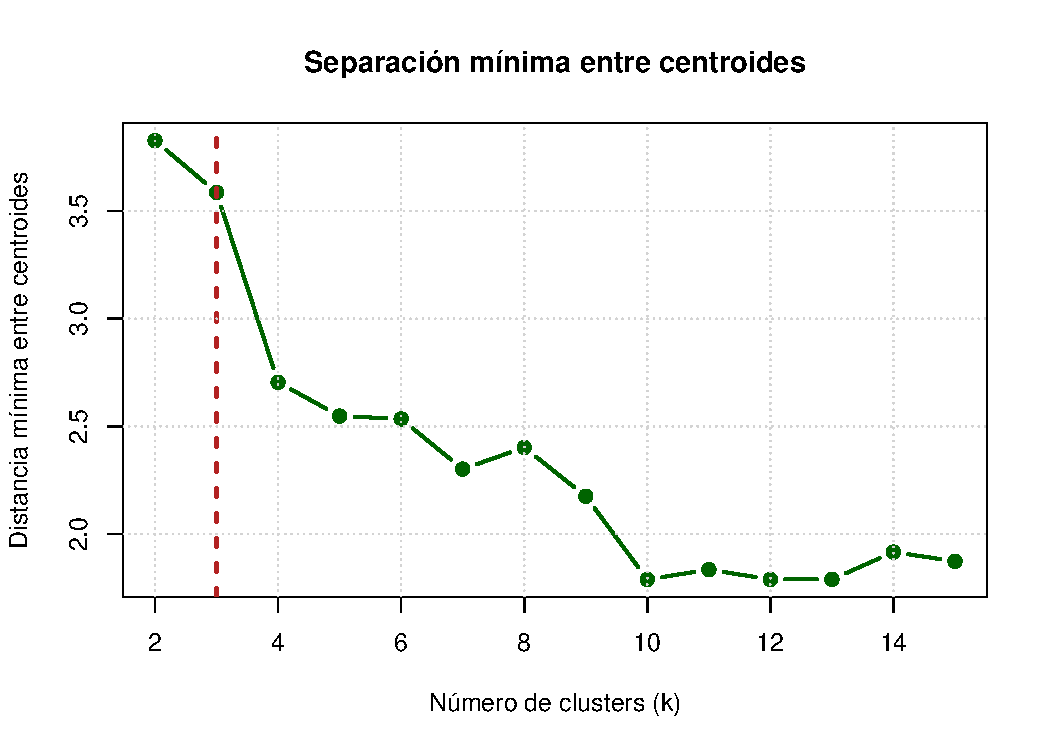
\includegraphics[width=0.75\textwidth]{cc4_diagnostico_dist_centroides.pdf}
  \caption{Diagnóstico 1: separación mínima entre centroides.}
  \label{fig:diagdist}
\end{figure}

\begin{figure}[H]
  \centering
  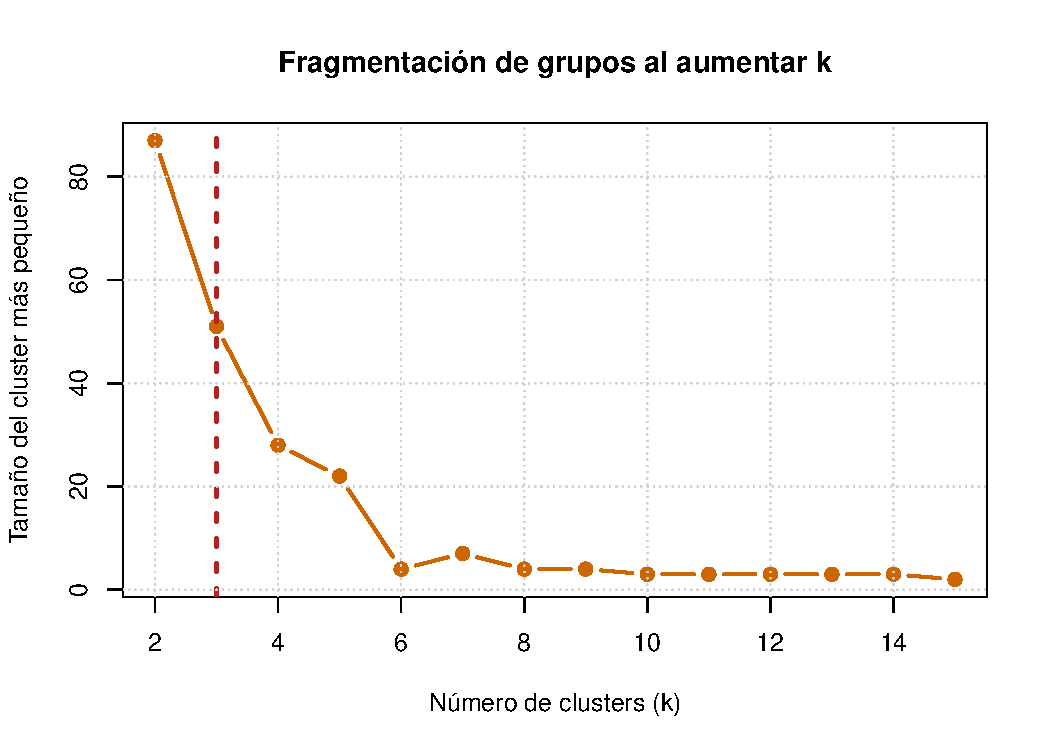
\includegraphics[width=0.75\textwidth]{cc4_diagnostico_tamano_cluster.pdf}
  \caption{Diagnóstico 2: tamaño del clúster más pequeño.}
  \label{fig:diagsize}
\end{figure}

\subsection*{A.2 Script R (procedimientos importantes)}
\phantomsection\label{anx:script}

\begin{lstlisting}
# Control 4 - INFO1184
set.seed(101)
wine <- read.csv("wine/wine.data", header = FALSE)
X <- scale(wine[, -1])

ks <- 2:15
wss <- sapply(ks, function(k) kmeans(X, centers = k, nstart = 100)$tot.withinss)

# Pregunta 1: diagnostico de centroides
diag_df <- data.frame(k = ks, min_centroid_dist = NA, min_cluster_size = NA)
for (i in seq_along(ks)) {
  km <- kmeans(X, centers = ks[i], nstart = 100, iter.max = 200)
  d <- as.matrix(dist(km$centers)); d[d == 0] <- NA
  diag_df$min_centroid_dist[i] <- min(d, na.rm = TRUE)
  diag_df$min_cluster_size[i] <- min(km$size)
}

# Pregunta 2: metodo del codo
plot(ks, wss, type = "b", pch = 19)
abline(v = 3, lty = 2, col = "red")
\end{lstlisting}

\subsection*{A.3 Bitácora de trabajo}
\phantomsection\label{anx:bitacora}

\begin{table}[H]
\centering
\footnotesize
\begin{tabular}{p{2.3cm} p{3.3cm} p{8.6cm}}
\toprule
Fecha & Actividad & Descripción \\
\midrule
22/04/2026 & Revisión de pauta y alcance & Se revisó el enunciado del control, la rúbrica general y el formato de entrega. Se definió el alcance del trabajo: responder la Pregunta 1 con evidencia basada en centroides/visualización y la Pregunta 2 con método del codo, sin mezclar criterios. \\
22/04/2026 & Revisión de clases y criterios técnicos & Se estudiaron las diapositivas de semana 6 para alinear el procedimiento con la metodología vista en curso. Se confirmó uso de k-medias con datos estandarizados, comparación de $k=2..15$ y justificación del $k$ óptimo con respaldo numérico y gráfico. \\
22/04/2026 & Implementación en R y generación de evidencia & Se ejecutó el script \texttt{CC4\_analisis.R} con semilla fija. Se calcularon métricas por cada $k$, se exportaron resultados a CSV y se generaron gráficos de PCA, codo y dos diagnósticos separados (distancia mínima entre centroides y tamaño del clúster más pequeño). \\
22/04/2026 & Interpretación y redacción del informe & Se contrastaron resultados de las dos preguntas y se validó consistencia de la conclusión ($k=3$). Luego se integraron tablas, figuras y referencias en \LaTeX{}, incorporando enlaces internos en anexos para facilitar la navegación y trazabilidad del análisis. \\
\bottomrule
\end{tabular}
\caption{Bitácora de actividades del control.}
\end{table}

\subsection*{A.4 Enlace a archivo .tex en Drive}
\phantomsection\label{anx:drive}
\href{https://drive.google.com/drive/folders/1XtYOXQIjELCpYi6g4Dtj3X43rOUEWrc1?usp=drive_link}{https://drive.google.com/drive/folders}

\end{document}
